\documentclass{article}
\usepackage{pgfplots}
    \pgfplotsset{
        compat=1.15,
    }
\begin{document}
    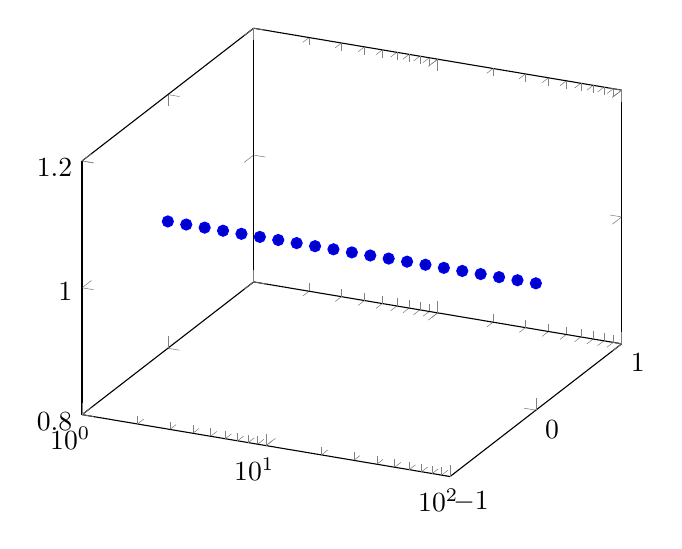
\begin{tikzpicture}
        \begin{axis}[
            only marks,
            domain=1:100,
            samples=21,
            samples y=1,
            xmode=log,
        ]
            \addplot3 {1};
        \end{axis}
    \end{tikzpicture}

    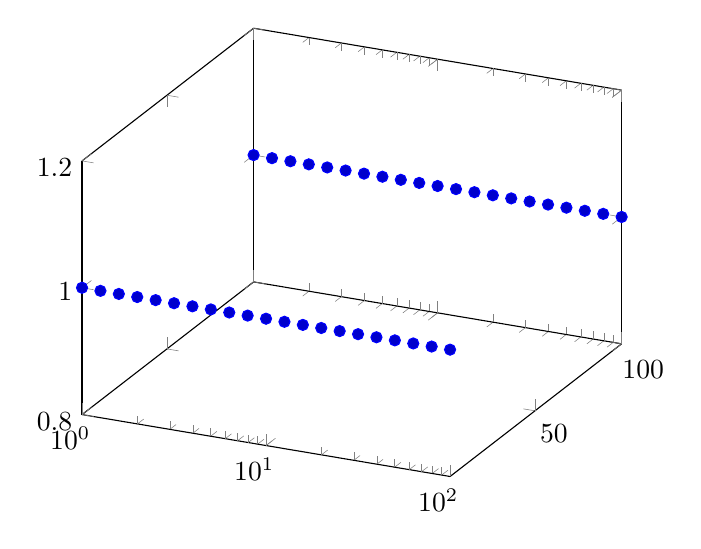
\begin{tikzpicture}
        \begin{axis}[
            only marks,
            domain=1:100,
            samples=21,
            samples y=2,
            xmode=log,
        ]
            \addplot3 {1};
        \end{axis}
    \end{tikzpicture}

    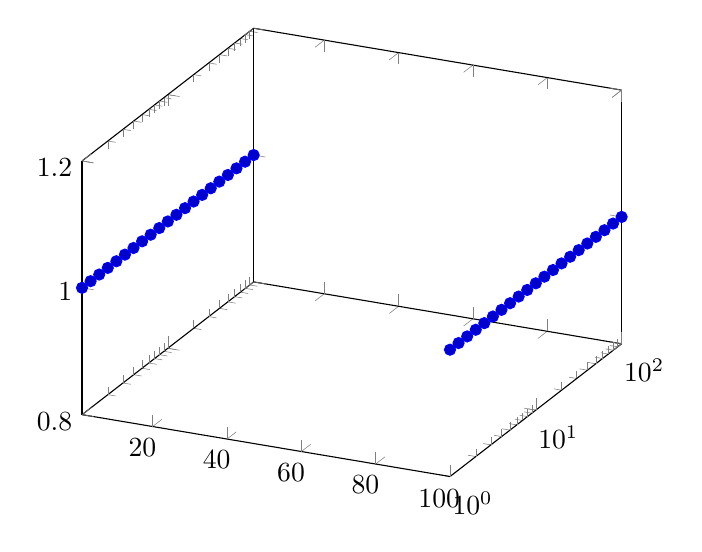
\begin{tikzpicture}
        \begin{axis}[
            only marks,
            domain=1:100,
            samples=2,
            samples y=21,
            ymode=log,
        ]
            \addplot3 {1};
        \end{axis}
    \end{tikzpicture}

    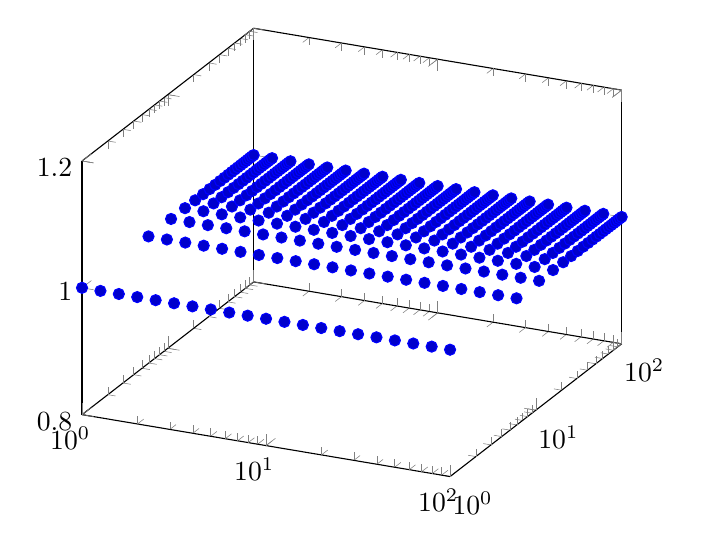
\begin{tikzpicture}
        \begin{axis}[
            only marks,
            domain=1:100,
            samples=21,
            samples y=21,
			xmode=log,
            ymode=log,
        ]
            \addplot3 {1};
        \end{axis}
    \end{tikzpicture}
\end{document}
